% Options for packages loaded elsewhere
\PassOptionsToPackage{unicode}{hyperref}
\PassOptionsToPackage{hyphens}{url}
%
\documentclass[
  12pt,
]{book}
\usepackage{amsmath,amssymb}
\usepackage{lmodern}
\usepackage{setspace}
\usepackage{iftex}
\ifPDFTeX
  \usepackage[T1]{fontenc}
  \usepackage[utf8]{inputenc}
  \usepackage{textcomp} % provide euro and other symbols
\else % if luatex or xetex
  \usepackage{unicode-math}
  \defaultfontfeatures{Scale=MatchLowercase}
  \defaultfontfeatures[\rmfamily]{Ligatures=TeX,Scale=1}
\fi
% Use upquote if available, for straight quotes in verbatim environments
\IfFileExists{upquote.sty}{\usepackage{upquote}}{}
\IfFileExists{microtype.sty}{% use microtype if available
  \usepackage[]{microtype}
  \UseMicrotypeSet[protrusion]{basicmath} % disable protrusion for tt fonts
}{}
\makeatletter
\@ifundefined{KOMAClassName}{% if non-KOMA class
  \IfFileExists{parskip.sty}{%
    \usepackage{parskip}
  }{% else
    \setlength{\parindent}{0pt}
    \setlength{\parskip}{6pt plus 2pt minus 1pt}}
}{% if KOMA class
  \KOMAoptions{parskip=half}}
\makeatother
\usepackage{xcolor}
\IfFileExists{xurl.sty}{\usepackage{xurl}}{} % add URL line breaks if available
\IfFileExists{bookmark.sty}{\usepackage{bookmark}}{\usepackage{hyperref}}
\hypersetup{
  pdftitle={Bayesian Inference for Species Distribution Modelling with Gaussian Processes},
  hidelinks,
  pdfcreator={LaTeX via pandoc}}
\urlstyle{same} % disable monospaced font for URLs
\usepackage[left=1in, right=1in, top=1in, bottom=1in]{geometry}
\usepackage{longtable,booktabs,array}
\usepackage{calc} % for calculating minipage widths
% Correct order of tables after \paragraph or \subparagraph
\usepackage{etoolbox}
\makeatletter
\patchcmd\longtable{\par}{\if@noskipsec\mbox{}\fi\par}{}{}
\makeatother
% Allow footnotes in longtable head/foot
\IfFileExists{footnotehyper.sty}{\usepackage{footnotehyper}}{\usepackage{footnote}}
\makesavenoteenv{longtable}
\usepackage{graphicx}
\makeatletter
\def\maxwidth{\ifdim\Gin@nat@width>\linewidth\linewidth\else\Gin@nat@width\fi}
\def\maxheight{\ifdim\Gin@nat@height>\textheight\textheight\else\Gin@nat@height\fi}
\makeatother
% Scale images if necessary, so that they will not overflow the page
% margins by default, and it is still possible to overwrite the defaults
% using explicit options in \includegraphics[width, height, ...]{}
\setkeys{Gin}{width=\maxwidth,height=\maxheight,keepaspectratio}
% Set default figure placement to htbp
\makeatletter
\def\fps@figure{htbp}
\makeatother
\setlength{\emergencystretch}{3em} % prevent overfull lines
\providecommand{\tightlist}{%
  \setlength{\itemsep}{0pt}\setlength{\parskip}{0pt}}
\setcounter{secnumdepth}{5}
\usepackage{booktabs}
\pagestyle{plain}
\ifLuaTeX
  \usepackage{selnolig}  % disable illegal ligatures
\fi
\usepackage[]{natbib}
\bibliographystyle{apalike}

\title{Bayesian Inference for Species Distribution Modelling with Gaussian Processes}
\usepackage{etoolbox}
\makeatletter
\providecommand{\subtitle}[1]{% add subtitle to \maketitle
  \apptocmd{\@title}{\par {\large #1 \par}}{}{}
}
\makeatother
\subtitle{Isaac William Caruso}
\author{Amherst College\\
Department of Computer Science}
\date{2021-04-08}

\usepackage{amsthm}
\newtheorem{theorem}{Theorem}[chapter]
\newtheorem{lemma}{Lemma}[chapter]
\newtheorem{corollary}{Corollary}[chapter]
\newtheorem{proposition}{Proposition}[chapter]
\newtheorem{conjecture}{Conjecture}[chapter]
\theoremstyle{definition}
\newtheorem{definition}{Definition}[chapter]
\theoremstyle{definition}
\newtheorem{example}{Example}[chapter]
\theoremstyle{definition}
\newtheorem{exercise}{Exercise}[chapter]
\theoremstyle{remark}
\newtheorem*{remark}{Remark}
\newtheorem*{solution}{Solution}
\begin{document}
\maketitle

{
\setcounter{tocdepth}{1}
\tableofcontents
}
\setstretch{1.7}
\hypertarget{probability-and-bayes-theorem}{%
\chapter{Probability and Bayes' theorem}\label{probability-and-bayes-theorem}}

This chapter provides an introduction to the probability concepts necessary to understand Bayesian inference.
Simply put, Bayesian inference is a statistical technique for estimating a quantity of interest upon the observation of data, while explicitly incorporating prior knowledge or belief about that quantity of interest.
Before embarking on an exposition of Bayesian statistics, we must first gain a basic understanding of a few key elements of probability theory---random variables, cumulative distribution functions, probability functions/ distributions, expected value, and conditional probability.
This chapter then concludes by introducing Bayes' theorem and Bayesian inference, and demonstrating the steps for performing a simple Bayesian update.

\hypertarget{random-variables}{%
\section{Random Variables}\label{random-variables}}

Imagine for a moment you are tossing a fair coin.
There are many experiments you could perform by tossing a coin, but let us consider our quantity of interest to be the fraction of times our coin lands on a tails.
It is clear that the number of tails, the outcome of our experiment, is dependent on the eventual realization of some random process.
A random variable \(X\) is a variable whose value is dependent on the outcome(s) of a stochastic phenomenon.
The realized value of \(X\) is denoted as \(x\).

In the example of tossing a coin, where the data is a sequence of coin tosses, e.g., \([H, T, T, …]\), we define the random variable \(X\) to be the number of tails.
If we toss the coin twice, \(X\) has three possible realized states, \(x\), depending on the outcome of this stochastic experiment: \(x = 0\), \(x = 1\), or \(x = 2\).
Table \ref{tab:rv} shows the probability that our random variable \(X\) takes value \(x\), some actual number of tails.

\begin{table}[!h]

\caption{\label{tab:rv}P(X = x) for two tosses}
\centering
\begin{tabular}[t]{rr}
\toprule
x & P(X = x)\\
\midrule
0 & 0.25\\
1 & 0.50\\
2 & 0.25\\
\bottomrule
\end{tabular}
\end{table}

The r.v. \(X\) is is an example of a \emph{discrete random variable}.
Discrete random variables can only assume discrete values.
To the contrary, continuous random variables are useful for describing continuous sample spaces.
For example, a continuous random variable may be used to represent the outcome of an experiment measuring blossoming heights of flowers, where the data is a sequence of observations of heights at which different flowers blossomed.
In this case, the outcome of our blossoming experiment can be any of an infinite number of real values, thus is properly modeled by a continuous random variable.

\hypertarget{cumulative-distribution-functions}{%
\section{Cumulative Distribution Functions}\label{cumulative-distribution-functions}}

In the previous example we represented the probability of various outcomes of a coin toss experiment in a tabular format.
Another way to represent this set of probabilities is as a \emph{cumulative distribution function}.

\begin{definition}[Cumulative distribution function 'CDF']
\protect\hypertarget{def:cdf}{}{\label{def:cdf} \iffalse (Cumulative distribution function `CDF') \fi{} }\emph{The cumulative distribution function is defined as a function where \(F_{X}\in[0, 1]\):}
\[F_{X}(x) \doteq P(X≤x)\]
\end{definition}

The cumulative distribution function \(F_{X}(x)\) simply represents the probability that a random variable \(X\) takes a value less than or equal to \(x\) for each possible input value of \(x\).
Figure \ref{fig:cdfimg} depicts a graphical representation of the CDF for our coin tossing experiment.



\begin{figure}

{\centering 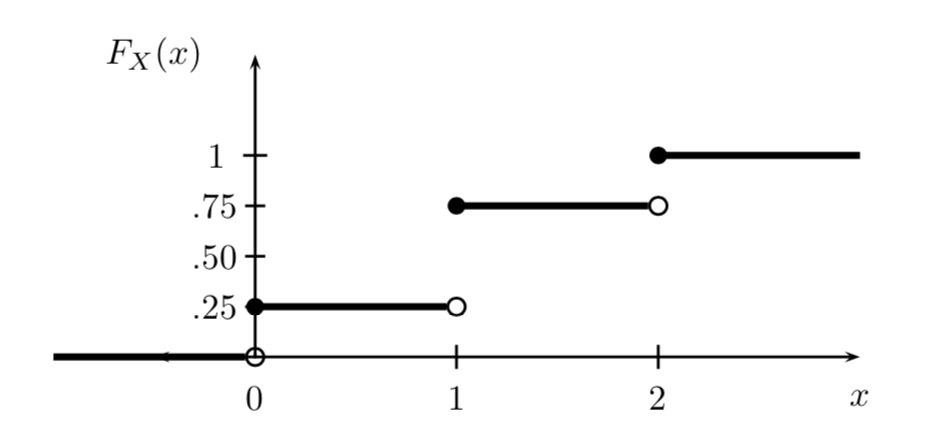
\includegraphics[width=0.7\linewidth]{./images/cdf} 

}

\caption{CDF for tossing a coin twice \citep{Wasserman2004}}\label{fig:cdfimg}
\end{figure}

Here, for every value of \(x\)---the number of tails in two coin tosses---the probability that \(X\) is equal to or less than this value is represented.
In this discrete example, we see that our CDF is represented by several non-decreasing discrete lines defined for all \(x\).
In the example of a continuous random variable, this function is a left-continuous, non-decreasing distribution also defined for all \(x\).

\hypertarget{probability-mass-and-density-functions}{%
\section{Probability Mass and Density Functions}\label{probability-mass-and-density-functions}}

The probability mass function and probability density function allow us to express probabilities of events over a sample space, and find their use with discrete and continuous random variables respectively.

In the discrete setting, the probability mass function for a random variable \(X\) yields the probability that \(X\) takes a value for every possible value that \(X\) can take.

\begin{definition}[Probability mass function 'PMF']
\protect\hypertarget{def:pmf}{}{\label{def:pmf} \iffalse (Probability mass function `PMF') \fi{} }\emph{The probability function for a discrete random variable \(X\)---the probability mass function for \(X\)---is defined as a function}
\[f_{X}(x) \doteq P(X=x)\]
\end{definition}

Here, the PMF has a few key attributes.
Namely \(P(X=x)>0\) for every \(x\) in the sample space \(S_{X}\) of \(X\), and \(\sum_{x \in S_{X}}f_{X}(x)=1\).
With these features in mind, the probability mass function of \(X\) follows logically from the cumulative distribution function of \(X\) insofar as the CDF is the sum of the PMF for all \(x_{i}≤x\), i.e., \[F_{X}(x) \doteq P(X≤x)=\sum_{x_i≤x}f_{X}(x_{i}).\]

In the case where the random variable \(X\) is continuous, its PDF is defined as follows.

\begin{definition}[Probability density function 'PDF']
\protect\hypertarget{def:pdf}{}{\label{def:pdf} \iffalse (Probability density function `PDF') \fi{} }\emph{The probability function for a continuous random variable \(X\)---the probability density function for \(X\)---is defined as a function \(f(x)\) where \(a\) and \(b\) are two real numbers such that \(a ≤ b\), so}
\[P(a<X<b) \doteq \int_{a}^{b}f_X(x)dx.\]
\end{definition}

In other words, the probability that the realized value \(x\) of our continuous random variable \(X\) is between two numbers \(a\) and \(b\) is equal to the integral of the probability density function of \(x\) from \(x = a\) to \(x = b\).
This formalization of the PDF \(f_X(x)\) allows a natural comparison with the CDF \(F_X(x)\) of \(X\),

\[F_X(x) \doteq \int_{-\infty}^{x}f_X(x)dx.\]

Specifically, this implies that \(F'_X(x)=f_X(x)\) for all differentiable points of \(F_X\).
In plain English this signifies that the derivative of the CDF is the PDF.

\hypertarget{expectation}{%
\section{Expectation}\label{expectation}}

One of the final core statistical concepts necessary to approach Bayesian statistics on sure footing is the idea of expectation or expected value.

\begin{definition}[Expectation]
\protect\hypertarget{def:e}{}{\label{def:e} \iffalse (Expectation) \fi{} }\emph{The expectation or expected value of a random variable X is}
\[E(X) \doteq \begin{cases}\sum_{x}xf_{X}(x) & \textrm{if }X\textrm{ is discrete}\\\int{xf_{X}(x)dx} & \textrm{if }X\textrm{ is continuous}\end{cases}\]
\end{definition}

To return to a familiar example, consider a random variable \(X\) to represent the number of tails in 6 coin tosses. Figure \ref{fig:binom} depicts the PMF for \(X\) using the \emph{binomial distribution} \(B(6,0.5)\) which represents the probability of observing a specific number of successes in a success-failure experiment.

\begin{figure}

{\centering 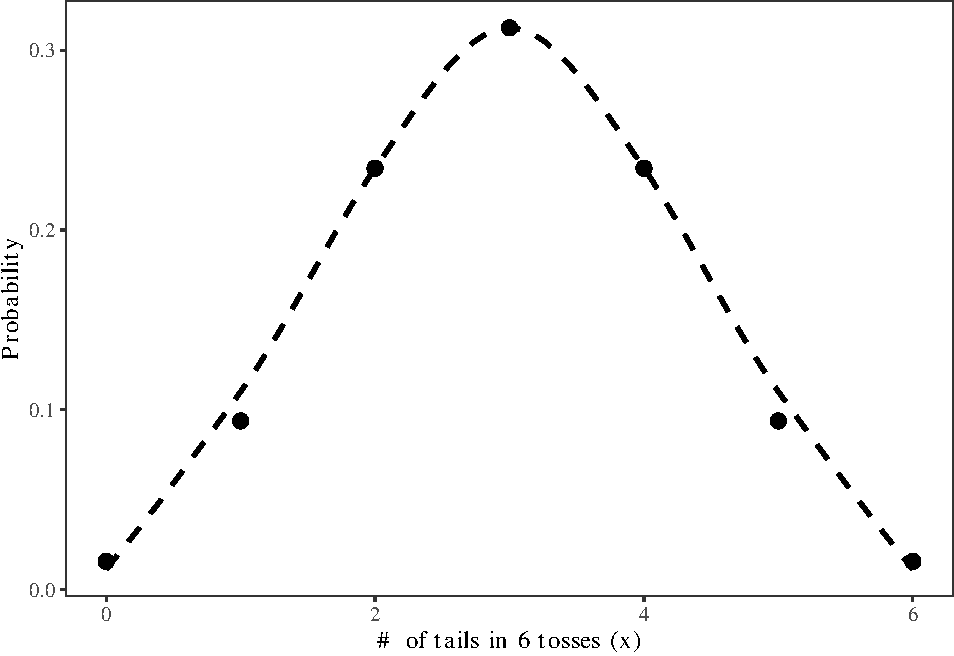
\includegraphics[width=0.5\linewidth]{manuscript_files/figure-latex/binom-1} 

}

\caption{The binomial probability mass function for the 6 trial coin toss experiment}\label{fig:binom}
\end{figure}

In this case, the x-axis represents each possible outcome \(x\) and the y-axis is the probability of that outcome. Table \ref{tab:bino} presents the value of the binomial PMF for every \(x \in X\).

\begin{table}[!h]

\caption{\label{tab:bino}P(X = x) for six tosses}
\centering
\begin{tabular}[t]{rr}
\toprule
x & y\\
\midrule
0 & 0.016\\
1 & 0.094\\
2 & 0.234\\
3 & 0.312\\
4 & 0.234\\
5 & 0.094\\
6 & 0.016\\
\bottomrule
\end{tabular}
\end{table}

Computing \(E(X)\) given the values in this table is demonstrated using the discrete case of Definition \ref{def:e} in Example \ref{exm:coin}.

\begin{example}
\protect\hypertarget{exm:coin}{}{\label{exm:coin} }The expected value of \(X \sim B(6, 0.5)\),
\[\begin{split}
E(X) & = \sum_{x}xf(x) \\
  & =  (0 \times 0.16)+(1 \times 0.094)+(2 \times 0.234)+(3 \times 0.312)\\
  & \;\;\;\; +(4 \times 0.234)+(5 \times 0.094)+(6 \times 0.016)\\
  & = 3
\end{split}\]
\end{example}

Importantly, while in this case \(E(X)\) corresponds well to the ``peak'' in the PMF, this should not be assumed to be the case unilaterally, as the same expectation would result from any distribution symmetrical about \(x=3\).

\hypertarget{conditional-probability}{%
\section{Conditional Probability}\label{conditional-probability}}

Conditional probability provides a way to model the probability that an event occurs, given that another event is known to have occured.
Conditional probability, as presented in Definition \ref{def:condprob}, requires only that the event assumed to have occured, i.e., the event we are \emph{conditioning on}, has a nonzero probability of occuring.

\begin{definition}[Conditional Probability]
\protect\hypertarget{def:condprob}{}{\label{def:condprob} \iffalse (Conditional Probability) \fi{} }\emph{Assuming \(P(B)>0\),}
\[P(A|B)=\frac{P(A \cap B)}{P(B)}\]
\end{definition}

Conditional probability asserts that the probability of event A occuring given that event B occurs is equivalent to the probability of both A and B occuring (denoted as \(A \cap B\)) divided by the probability that B occurs. \(P(A|B)\) is not generally equal to \(P(B|A)\)
For example, the probability that I am swimming given that I am in the water is clearly not the same as the probability that I am in the water given that I am swimming.
Example \ref{exm:condprobe} explains how to use conditional probability to calculate the probability of rolling a 2 on a 6-sided dice, given I know the outcome of the roll is less than 4.

\begin{example}
\protect\hypertarget{exm:condprobe}{}{\label{exm:condprobe} }Conditional probability can be used to determine the probability of rolling a 2 on a 6 sided dice, given that I know the outcome will be less than 4. This scenario can be represented as:
\[A = \textrm{rolls 2, } P(A) = 1/6\]
\[B = \textrm{rolls < 4, } P(B) = 4/6\]
\[\begin{split}
P(2|<4) = P(A|B) & = \frac{P(A \cap B)}{P(B)} \\
  & = \frac{\frac{1}{6}\frac{4}{6}}{\frac{4}{6}} \\
  & = \frac{1}{6}
\end{split}\]
\end{example}

\hypertarget{bayes-theorem-for-discrete-values}{%
\section{Bayes' Theorem for Discrete Values}\label{bayes-theorem-for-discrete-values}}

Consider a student, Alice, who was exposed to someone with COVID-19.
Being a responsible person, Alice decides she should get tested.
She receives a test and the accompanying information sheet states the test is 85\% accurate, meaning that 85\% of the time it gives positive results to recipients who are actually positive. The sheet also says that the test yields a false positive 30\% of the time, meaning that if Alice is actually negative she will still receive a positive test 30\% of the time.
The following day Alice receives a positive test.
As a student of probability, Alice recognizes that the 85\% accuracy statistic only means the conditional probability that she receives a positive test given she is COVID positive (\(P(+ test|covid+)\)) is 85\%.
However, Alice is actually interested in the conditional probability that she is positive given she just tested positive, \(P(covid+|test+)\).
As stated in the previous section's discussion of conditional probability, \(P(A|B) \neq P(B|A)\).
Bayes' theorem, which follows intuitively from the theorem of conditional probability, provides this answer for Alice.
We can rewrite Definition \ref{def:condprob} as
\[P(A \cap B)=P(A|B)P(B).\]
Furthuremore, it can also be stated that
\[P(B \cap A)=P(B|A)P(A)\]
Clearly \(P(A \cap B)=P(B \cap A)\), as both terms can be used interchangeably to represent the intersection of two sets A and B.
This equivalency means that we can rewrite these equations as
\[P(B|A)P(A)=P(A|B)P(B)\]
Dividing both sides of this equivalency by \(P(B)\) yields Bayes' theorem, as formalized in Definition \ref{def:bayestheorem} \citep{Junker2003}.

\begin{definition}[Bayes' Theorem]
\protect\hypertarget{def:bayestheorem}{}{\label{def:bayestheorem} \iffalse (Bayes' Theorem) \fi{} }\emph{Assuming \(P(B)>0\) and \(P(A)>0\),}
\[P(B|A)=\frac{P(A|B)P(B)}{P(A)}\]
\end{definition}

Additionally, the \emph{law of total probability}, Definition \ref{def:totprob}, can be used to compute \(P(A)\) for a discrete sample space \(S_{B}\) \citep{Wasserman2004}.

\begin{definition}[Law of Total Probability]
\protect\hypertarget{def:totprob}{}{\label{def:totprob} \iffalse (Law of Total Probability) \fi{} }\emph{\(B_{0},...,B_{k}\) is a partition of a discrete sample space \(S_{B}\), and}
\[P(A)=\sum_{i=1}^{k}P(A|B_{i})P(B_{i}).\]
\end{definition}

Returning to our example, the partition of this sample space is \([B_{0}=covid+,\textrm{ } B_{1}=covid-]\), as Alice is either COVID positive or she is not.
The final piece of information needed is the prior probability \(P(B)\), which can be thought of as the likelihood of contracting covid from any given exposure.
Alice did some research and concluded this likelihood is 20\%.
Given the information from the factsheet and Alice's prior knowledge about the probability of contracting covid, Example \ref{exm:covid} shows how Alice can use Bayes' theorem to answer her question and find the probability that she is actually positive given she has tested positive.

\begin{example}
\protect\hypertarget{exm:covid}{}{\label{exm:covid} }Given the following information:
\[P(test+|covid+)=0.85 \textrm{, } P(test+|covid-)=0.30 \textrm{, } P(covid+)=0.20 \textrm{, } P(covid-)=0.80\]
We can represent the conditional probability that Alice is COVID positive given that she tested positive \(P(covid+|test+)\) as
\[\begin{split}
P(covid+|test+) & = \frac{P(test+|covid+)P(covid+)}{P(test+|covid-)P(covid-)+P(test+|covid+)P(covid+)}\\
& = \frac{(0.85)(0.20)}{(0.30)(0.80)+(0.85)(0.20)} \\
& = \frac{0.17}{0.24+0.17} \\
& = 0.41
\end{split}\]
\end{example}

\hypertarget{bayes-theorem-for-probability-distributions}{%
\section{Bayes' Theorem for Probability Distributions}\label{bayes-theorem-for-probability-distributions}}

While Bayes' theorem can be correctly applied to discrete values, evaluating Bayes' theorem for probability distributions as an alternative to discrete values will allow uncertainty to be represented in a natural manner.
In the previous example, we considered the prior probability that Alice contracts COVID in any given exposure to be an exact value of 0.20.
Given that the virus that causes COVID-19 is not well understood at present moment, this value is clearly not an accurate representation of the uncertainty related to our prior knowledge as different sources may give varying values for this prior plausibility.
Considering Bayes' theorem in terms of probability distributions will remove this assumption from the model in favour of a probability distribution, which represents a weighted range of all possible values of our parameter as highlighted in Definition \ref{def:bayesprob}.

\begin{definition}[Bayes' Theorem for Probability Distributions]
\protect\hypertarget{def:bayesprob}{}{\label{def:bayesprob} \iffalse (Bayes' Theorem for Probability Distributions) \fi{} }\emph{Assuming \(P(\theta)>0\) and \(P(X)>0\),}
\[P(\theta|X)=\frac{P(X|\theta)P(\theta)}{P(X)},\]
\end{definition}
where \(P(\theta|X)\) is the posterior probability, \(P(\theta)\) is the prior probability distribution of the parameter of interest \(\theta\), \(P(X|\theta)\) is the likelihood function or the probability of the data given \(\theta\), and \(P(X)\) is the marginal likelihood of the data \(X\).
In this case, the marginal likelihood \(P(X)\) functions to normalize the posterior distribution and is evaluated for a continuous sample space as:
\[P(X)=\int P(X|\theta)P(\theta)d\theta\]

\hypertarget{approximation-algorithms-for-inference-on-distributions}{%
\chapter{Approximation algorithms for inference on distributions}\label{approximation-algorithms-for-inference-on-distributions}}

When performing Bayesian Inference, approximation algorithms are necessary for updating the relative probability of parameters of interest in a computationally feasible manner.
In modelling scenarios with multiple parameters forming a multidimensional parameter space, evaluating parameters at even a relatively small number of possible values rapidly becomes intractible.
This problem is further exaggerated in the evaluation of hierarchical models, which are of particular interest in many application domains including biology, economics, chemistry, and physics.
Here, we discuss markov chain monte carlo based sampling algorithms, which allow for efficiently sampling from approximations of probability distributions.

\hypertarget{markov-chain-monte-carlo}{%
\section{Markov Chain Monte Carlo}\label{markov-chain-monte-carlo}}

Markov chain monte carlo (MCMC) provides an efficient methodology for sampling from the posterior curve to perform a Bayesian update. We will first provide a theoretical background into markov chains and monte carlo approximation, followed by a discussion of \emph{Metropolis-Hastings Monte Carlo}, an algorithm for performing MCMC.

\hypertarget{markov-chains}{%
\subsection{Markov Chains}\label{markov-chains}}

A markov chain is a stochastic model expressing a sequence of possible states in which the probability of each state, \(X_{i-1}\), depends only on the value attained in the previous state, \(X_{i-1}\).
A markov chain has several properties which are essential for its application in Bayesian statistics.
Namely, each state in the chain depends only on the previous one; therefore, the markov chain preserves the assumed dependence between samples from our posterior distribution.
Additionally, this localized dependence lends the markov chain another attractive feature in that it is effectively memoryless.
Definition \ref{def:markov} formalizes the requirements for a markov chain \citep{Wasserman2004}.

\begin{definition}[Markov Chain]
\protect\hypertarget{def:markov}{}{\label{def:markov} \iffalse (Markov Chain) \fi{} }\emph{A discrete sequence of random variables \({X_{0},X_{1},...,X_{i}}\) is a Markov chain iff it satisfies the Markov property; that is, for all \(i\) and \(x \in X\):}
\[P(X_{i}=x|X_{0},...X_{i-1})=P(X_{i}=x|X_{i-1})\]
\end{definition}

A markov chain is often represented as a directed graph where states in the sequence of random variables are represented as vertices, and edges represent possible paths between states whose weights are the probabilities of edges being traversed.

\hypertarget{monte-carlo-approximation}{%
\subsection{Monte Carlo Approximation}\label{monte-carlo-approximation}}

Monte Carlo approximation provides a convient method for approximately computing quantities of interest.
This schema will allow for drawing samples from arbitrarily complex probability distributions.
The basic example, known as monte carlo integration, evaluates an integral using monte carlo approximation \citep{Wasserman2004}.
If we want to evaulate an integral for some function \(f(x)\), where
\[I=\int_{a}^{b}f(x)dx \textrm{ ,}\]
we can approximate \(I\) using monte carlo approximation. \(f(x)\) can be alternatively expressed as two functions, \(h(x)\) and \(w(x)\), where \(h(x)=\frac{1}{a-b}\) and \(w(x)=f(x)(b-a)\) as follows.
\[I=\int_{a}^{b}f(x)dx=\int_{a}^{b}w(x)h(x)dx\]
Conveniently, \(h\) is a pdf of a uniform r.v. \(X\) over \([a,b]\), which means that \(I\) can be rewritten in terms of expectation as
\[I=E_{f}(w(X)) \textrm{ .}\]
In conjunction with the law of large numbers, this means that if we generate a sequence of random variables from a uniform distribution \(X_{0},...,X_{N}\sim unif(a,b)\) then the standard Monte Carlo integration method asserts

\[\hat{I}\equiv\frac{1}{N}\sum_{i=0}^{N}w(X_{i})\rightarrow E(w(X))=I \textrm{ .}\]

In other words, \(\hat{I}\) approaches \(I\) as \(N\) grows sufficiently large.
Constructing a Markov chain for evaluation with Monte Carlo will maintain the inherent, presumed dependence between samples of a sequence of random variables while facilitating the random sampling of extremely complex probability distributions.
As we will expand on in the following sections, this algorithmic framework is particularly useful because it will work for models with non-normal posteriors, including hierarchical models.

\hypertarget{metropolis-hastings-mcmc}{%
\section{Metropolis-Hastings MCMC}\label{metropolis-hastings-mcmc}}

\emph{Metropolis-Hastings MCMC} is one common algorithm for sampling from the posterior distribution to perform a Bayesian update.
While it is not always the fastest in practice and requires manual tuning to work effectively, Metropolis-Hastings provides a foundation for more complex algorithms such as \emph{Hamiltonian Monte Carlo} with \emph{No-U-Turn sampling}.
To reiterate, the purpose of sampling in Bayesian inference is to draw from some density for parameters theta.
In this case, the density we are drawing from is the Bayesian posterior \(P(\theta|data)\), which for the purposes of MCMC is referred to as the \emph{target distribution}.
Metropolis-Hastings algorithm provides a method for sampling from an approximation of the target distribution known as the \emph{stationary distribution}.
Critically, the law of large numbers guarantees that with sufficiently many iterations of Metropolis-Hastings, the stationary distribution will converge on the target distribution and samples drawn from the stationary distribution will appear to be samples from the target distribution.
Essentially, given some sequence of states \(X_{0},X_{1},...,X_{i}\) from a Markov-Chain, where \(X_{0}\) is chosen arbitrarily, an iteration of Metropolis-Hastings produces the next state to include in the sequence.
As presented formally in Definition \ref{def:methas}, this is achieved by generating a \emph{proposal} for \(X_{i+1}\) from the \emph{proposal distribution} \(q(y|X_{i})\), transition kernel, and then accepting the proposal with some probability dependent on the relative, target probabilities of the current state \(X_{i}\) and the proposal \citep{Wasserman2004}.

\begin{definition}[Metropolis-Hastings MCMC]
\protect\hypertarget{def:methas}{}{\label{def:methas} \iffalse (Metropolis-Hastings MCMC) \fi{} }\emph{\(X_{i+1}\) is generated given \(X_{0},X_{1},...,X_{i}\) in the following manner:}

\begin{enumerate}
  \item Sample a proposal $Y$ from the proposal distribution $Y \sim q(y|X_{i}) \textrm{ .}$
  \item Evaulate the ratio of probabilities in the stationary distribution $h(x)$ for $r(X_{i},Y)$ where $$ r(x,y)=min \{\frac{f(y)}{f(x)} \frac{q(x|y)}{q(y|x)} ,1 \} \textrm{ .}$$
  \item Compute the next state $X_{i+1}$, where $$X_{i+1}=\begin{cases}Y & \textrm{with probability }r \\ X_{i} & \textrm{with probability }1-r \end{cases} \textrm{ .}$$
\end{enumerate}
\end{definition}

A simplification of the acceptance probability \(r(x,y)\) occurs in a special case of Metropolis-Hastings known as random walk Metropolis-Hastings, where the proposal distribution is a standard normal distribution \(N(0,1)\).
This case is a random walk because the proposal \(Y\) is generated by adding a random number sampled from a standard normal distribution to \(X_{i}\).
When the proposal distribution is a symmetric distribution---as is the case with the normal distribution---\(q(y|x)=q(x|y) \therefore \frac{q(x|y)}{q(y|x)}=1\) .
This means that the acceptance probability can be simplified as follows. \[r(x,y)=min \{\frac{f(y)}{f(x)},1 \}\]

While Metropolis-Hastings may seem appealing because it is both memoryless and able to approximate very complex distributions, its downfall lies in the manual tuning and iteration necessary to achieve convergence of the stationary distribution to the target distribution in a reasonable number of iterations.
Recall that Metropolis-Hastings generates proposals by sampling from some distribution, and in the case of random walk metropolis this is a normal distribution centered about \(X_{i}\).
Here, the standard deviation of the normal distribution, known as the step size, dictates the relative distance in the sample space between \(X_{i}\) and the generated proposal.
If the step size is too low, the algorithm will make very small steps and may miss key features of the target distribution, causing the stationary distribution to require a much larger number of iterations to converge on the target distribution.
On the other hand if the step size is too large, proposals will be overwhelmingly generated from the low-probability tails of the distribution, again resulting in a lack of convergence and poorly representative samples from the stationary distributon.
While some methods have been proposed for automatically tuning the step size parameter \citep{Graves2011}, iterating on complex, Bayesian models to tune a parameter is not particularly efficient nor computationally feasible in many cases.
For this reason, other approximation algorithms are used in practical implementations of Bayesian inference.
One such algorithm, \emph{Hamiltonian Monte Carlo} (HMC), relies on theorhetical physics to compute a latent momentum variable which is applied to a hamiltonian, effectively simulating a ball rolling around the multi-dimensional sample space \citep{Brooks2011}.
Despite the increased computational cost, this method is appealing because of its ability to generate proposals from distant regions of the stationary distribution with high acceptance probabilities.
This means that in practice, the HMC algorithm's stationary distribution converges on the target distribution with far fewer iterations than traditional Metropolis-Hastings implementations.
Though HMC still requires the user to specify a step size as well as a number of steps to move the hamiltonian before considering a proposal, in practice it is much more efficient and requires fewer iterations on a model.
Additionally, a proposed extension to HMC called the \emph{No-U-Turn Sampler} (NUTS) automatically determines the number of steps and was empirically demonstrated to perform at least equally as well as standard HMC \citep{Homan2014}.
The approximation algorithms breifly covered in this chapter underpin modern applications for Bayesian inference, including STAN, which are discussed in the following chapter.

\hypertarget{modern-bayesian-inference-with-stan}{%
\chapter{Modern Bayesian inference with STAN}\label{modern-bayesian-inference-with-stan}}

\hypertarget{bayesian-applications-in-biology-hybrid-species-distribution-modelling-with-gaussian-processes}{%
\chapter{Bayesian applications in Biology: Hybrid species distribution modelling with gaussian processes}\label{bayesian-applications-in-biology-hybrid-species-distribution-modelling-with-gaussian-processes}}

  \bibliography{references.bib,packages.bib}

\end{document}
